\section{Anwendungen der NMR}
Die NMR fidnet in vielen unterschiedlichen Bereichen Anwendung, wesegen hier 3 verschiedene Anwendungen der NMR vorgestellt und erläutert werden sollen.

\subsection{NMR in der Medizin (MRT)}
Die Magnetresonanztomografie (MRT) ist ein bildgebendes Verfahren zur Darstellung von Organen oder Gewebe des Körpers. Ausgenutzt wird dabei der Kernspin der Protonen, sodass die Protonendichte oder unterschiedliche Relaxationszeiten die unterschiedlichen Gewebearten bzw. Kontraste darstellen.
\subsubsection*{Aufbau einer typischen Anlage zur MRT}
\begin{figure}[htbp] 
     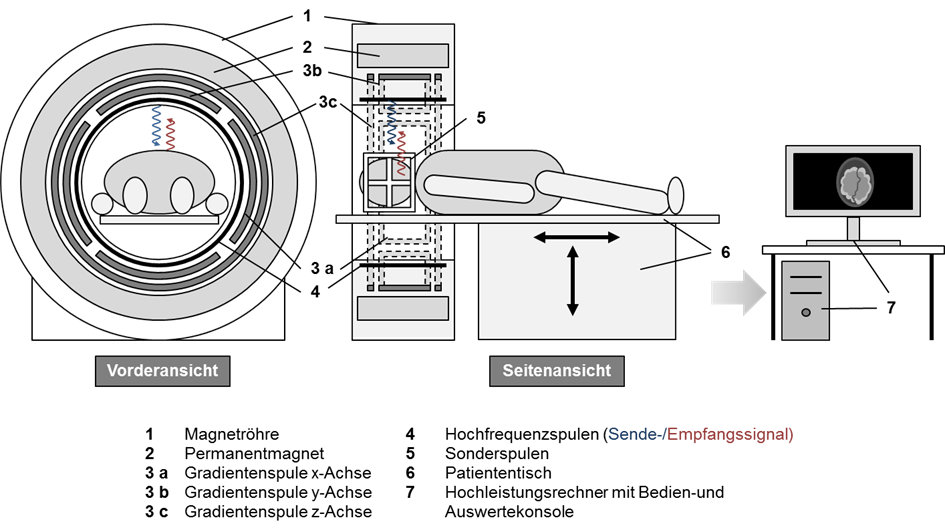
\includegraphics[width=0.99\textwidth]{mrt_aufbau.png}
  \caption{Schematischer Aufbau einer MRT-Anlage \cite{mrt}}
  \label{mrt_aufbau}
\end{figure}
In Abblidung \ref{mrt_aufbau} sieht man den Aufbau einer typischen MRT-Anlage. Die entscheidenden Elemente sind Gradientenspulen und die Hochfrequenzspulen, sowie der Permanentmagnet, der die Aufpaltung der Kernspinlevel der Protonen verursacht.
\subsubsection*{Funktionsprinzip der MRT}
Der Permanentmagnet ist ein supraleitender mit Helium gekühlter Magnet, der ein nahezu räumlich konstantes Magnetfeld von $1,5T$ oder $3T$ liefert. Durch die Hochfrequenzspule wird die Magnetisierung des Patienten kurzzeitig verändert, der Übergang in die ursprüngliche Magnetisierung erfolgt dann durch Aussenden Strahung, welche von der Hochfrequenzspule empfangen wird. Die räumliche Zuordnung erfolgt durch die Gradientenspulen, die in x-, y-, und z-Richtung ausgerichtet sind. DIe Sonderspulen verbessern das Signal und am Hochleistungsrechner wird dann aus den Daten das Bild erstellt. 

\subsection{NMR in der Chemie (Strukturanalyse)}
In der Chemie wird die NMR genutzt, um die Struktur von Molekülen genauer zu untersuchen. Entscheidend ist, dass die Resonanzen in unterschiedlichen Bindungen in ihrer Frequenz unterschiedlich verschoben werden.
\subsubsection*{Chemische Verschiebung}
Die Elektronen, die den Atomkern umgeben, bewegen sich entsprechend dem angelegten Magnetfeld $B_0$, da sie geladene Teilchen sind. So generieren sie ein viel kleineres entgegengerichtetes Magnetfeld, was den Kern vom Magnetfeld teilweise abschirmt. $B_0$ muss also leicht erhöht werden, damit Resonanz bei einer gegebenen Radiofrequenz auftritt. Unterschiedliche Bindungen führen zu unterschiedlichen Abschirmungen, sodass die Verschiebung des Magnetfelds spezifisch zu ein Referenz in $ppm$ angegeben werden kann. In Protonen-NMR wird als Referenz Tetramethylsilan (TMS) verwendet, da einen scharfen Peak im Spektrum hat und weitere positive chemische Eigenschaften besitzt.
\subsubsection*{Kopplungsstruktur der NMR-Spektren}
In der Wasserstoff-NMR-Spektroskopie tritt ein Effekt auf, der durch das Koppeln der benachbarten Protonen entsteht. Das benachbarte Proton kann einen zum angelegten Magnetfeld parallelen oder antiparallelen Kernspin haben. Dadurch teilt sich der Zustand des anderen Protons zu einem Dublett auf. Ganz allgemein ergeben sich für $n$ Nachbarn $ n + 1$ neue Zustände, die im NMR-Spektrum zu sehen sind.

\subsection{NMR in der Festkörperphysik}
\subsubsection*{Besonderheiten der Festkörper-NMR}
Für Materialien, in denen die Atome oder Moleküle keine oder nur eine sehr geringe Beweglichkeit haben, können die richtungsabhängigen Interaktionen der einzelnen Atomkerne mit Hilfe der NMR-Spektroskopie aufgelöst werden. Anders gesagt verändern die richtungsabhängigen Interaktionen die Kernspin-Energielevels.
\subsubsection*{Magic-Angle-Spinning-NMR}
Durch die eben beschriebenen anistropen Wechselwirkungen treten Linienverbreiterungen auf, die es erschweren, das NMR-Spektrum zu analysieren. Eine Methode, um die Signalqualität zu verbessern ist das Magic-Angle-Spinning (MAS). Dabei wird die Probe um eine Rotationsachse rotiert, die in einem Winkel von ca. $54,74°$ zu dem externen Magnetfeld ausgerichtet ist. Die anisotropen Wechselwirkungen können so herausgemittelt werden und die Linienbreiten des Spektrums wird deutlich schärfer.
\subsubsection*{Knight-Shift}
Der Knight-Shift ist ein Effekt, der auftritt, wenn man die Resonanzfrequenz von einem Atom in einem Nichtmetall und in einem Metall vergleicht. Ähnlich wie bei der chemischen Verschiebung wird dem äußeren Magnetfeld ein effektives Magnetfeld überlagert, was durch die Ausrichtung der Spins der Leitungselektronen entsteht, wenn ein externes Magnetfeld angelegt ist. So wird die Resonanzfrequenz um einen Betrag der Größenordnung ein Promille verschoben.

